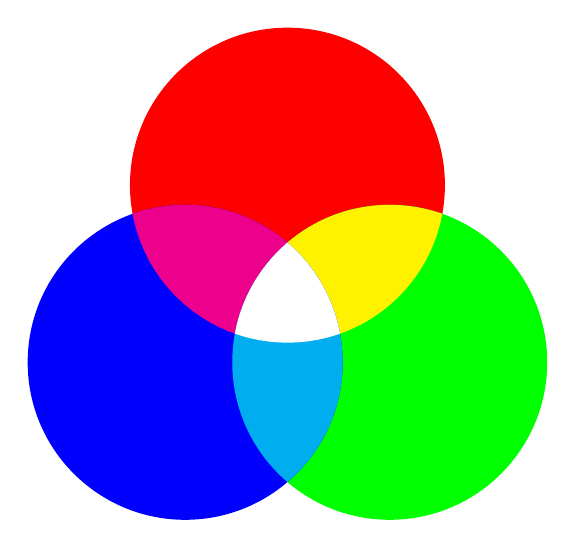
\begin{tikzpicture}

  \draw [draw=none, fill=red] (90:1.5) circle (2cm);
  \draw [draw=none, fill=green] (-30:1.5) circle (2cm);
  \draw [draw=none, fill=blue] (210:1.5) circle (2cm);

  \begin{scope}
    \clip (90:1.5) circle(2cm);
    \draw [draw=none, fill=yellow] (-30:1.5) circle (2cm);
  \end{scope}

  \begin{scope}
    \clip (210:1.5) circle(2cm);
    \draw [draw=none, fill=magenta] (90:1.5) circle (2cm);
  \end{scope}

  \begin{scope}
    \clip (-30:1.5) circle(2cm);
    \draw [draw=none, fill=cyan] (210:1.5) circle (2cm);
  \end{scope}

  \begin{scope} % red + green + blue = white
    \clip (90:1.5) circle(2cm);
    \clip (210:1.5) circle(2cm);
    \draw [draw=none, fill=white] (-30:1.5) circle (2cm);
  \end{scope}
\end{tikzpicture}
